\documentclass{standalone}
\usepackage{tikz}
\usepackage{pgfplots}
\pgfplotsset{compat=1.18}
\begin{document}


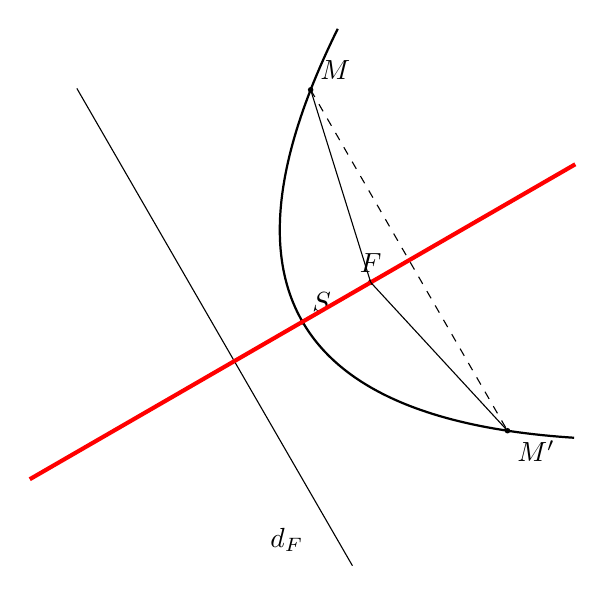
\begin{tikzpicture}

% Parameters
\def\xC{4}    % vertex x
\def\yC{1.5}  % vertex y
\def\p{1}     % focal length
\def\ang{30}  % rotation angle in degrees

% Axis vector for symmetry
\pgfmathsetmacro{\cosA}{cos(\ang)}
\pgfmathsetmacro{\sinA}{sin(\ang)}

% Parabola y^2 = 4px in local coordinates (x along axis)
\draw[thick, rotate around={\ang:(\xC,\yC)}, domain=-3:3, samples=100]
    plot ({\xC + (\x*\x)/(4*\p)}, {\yC + \x});

% Vertex
\fill (\xC,\yC) circle (1pt) node[above right] {$S$};

% Focus
\coordinate (F) at ({\xC + \p*cos(\ang)},{\yC + \p*sin(\ang)});
\fill (F) circle (1pt) node[above] {$F$};

% Directrix
\draw[thin, rotate around={\ang:(\xC,\yC)}]
    ({\xC-\p},{\yC-3}) -- ({\xC-\p},{\yC+4});
\node[below left] at ({\xC+1-\p*cos(\ang)},{\yC-2-\p*sin(\ang)}) {$d_F$};

% Axis of symmetry
\draw[red, line width =1.5pt] 
    (\xC - 4*\cosA, \yC - 4*\sinA) -- (\xC + 4*\cosA, \yC + 4*\sinA);

% Pick a point M in local coordinates (y_local)
\def\yM{2.5} % perpendicular distance from axis
\pgfmathsetmacro{\xM}{(\yM*\yM)/(4*\p)} % x coordinate along axis
% Rotate M around vertex
\coordinate (M) at 
({\xC + \xM*\cosA - \yM*\sinA},
 {\yC + \xM*\sinA + \yM*\cosA});
\fill (M) circle (1pt) node[above right] {$M$};

% Mirror point M' across axis
\coordinate (Mp) at
({\xC + \xM*\cosA + \yM*\sinA},
 {\yC + \xM*\sinA - \yM*\cosA});
\fill (Mp) circle (1pt) node[below right] {$M'$};

% Lines from focus to points
\draw[-] (F) -- (M);
\draw[-] (F) -- (Mp);

% Segment connecting M and M'
\draw[dashed] (M) -- (Mp);

\end{tikzpicture}
\end{document}